% Part: sets-functions-relations
% Chapter: relations
% Section: graphs

\documentclass[../../../include/open-logic-section]{subfiles}

\begin{document}

\olfileid[zh]{sfr}{rel}{grp}
\olsection{图}

\emph{图}（graph）是一种图式，其中的点——称为「节点」或
「顶点」（「vertex」的复数）——由边连接起来。图是离散数学和计算机
科学中无处不在的工具。它们对于表示和可视化关系与结构极为有用，从
诸如各种网络这样的具体事物，到像决策的可能结果这样的抽象结构。文献
中有许多不同种类的图，它们各不相同，例如，取决于边是否有向、是否有
标记，是否有从一个节点到同一节点的边，同一对节点之间是否有重边，等
等。\emph{有向图}与关系有着特殊的关联。

\begin{defn}[有向图]
\emph{有向图} $G = \tuple{V, E}$ 是一个\emph{顶点}~$V$ 的集合和
一个\emph{边}的集合 $E \subseteq V^2$。
\end{defn}

\begin{explain}
根据我们的定义，图就是集合连同该集合上的一个关系。当然，在谈及图时，
自然期望它们被图示出来：我们可以把一个图绘制成当且仅当
$\tuple{v_1, v_2} \in E$ 时用箭头连接两个顶点~$v_1$ 和 $v_2$。
关系本身与图的唯一区别在于，图规定了顶点集合，即一个图可能含有孤立
的顶点。然而，重要的是，集合~$X$ 上的每一个关系~$R$ 都可以被看作有向
图 $\tuple{X, R}$，反过来，有向图~$\tuple{V, E}$ 也可以被看作关系
$E \subseteq V^2$，并且集合 $V$ 被显式地规定。
\end{explain}

\begin{ex}
具有 $V = \{1, 2, 3, 4\}$ 和 $E =
\{\tuple{1,1}, \allowbreak \tuple{1, 2}, \allowbreak \tuple{1, 3},
\allowbreak \tuple{2, 3}\}$ 的图 $\tuple{V, E}$ 如下图所示：
\begin{align*}
& 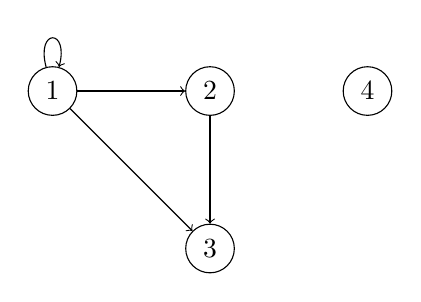
\begin{tikzpicture}[->,node distance=2cm]
  \node[draw,circle] (A) {$1$};
  \node[draw,circle] (B) [right of=A] {$2$};
  \node[draw,circle] (C) [below of=B] {$3$};
  \node[draw,circle] (D) [right of=B] {$4$};
  \draw (A) to [loop above]  (A);
  \draw (A) to  (B);
  \draw (A) to  (C);
  \draw (B) to  (C);
  \end{tikzpicture}
\intertext{这与具有 $V' =
  \{1, 2, 3\}$ 的图 $\tuple{V', E}$ 是不同的图，后者如下图所示：}
& 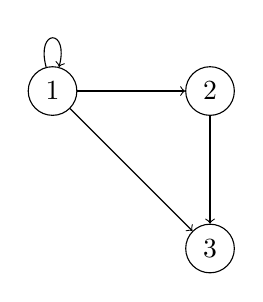
\begin{tikzpicture}[->,node distance=2cm]
  \node[draw,circle] (A) {$1$};
  \node[draw,circle] (B) [right of=A] {$2$};
  \node[draw,circle] (C) [below of=B] {$3$};
  \draw (A) to [loop above]  (A);
  \draw (A) to  (B);
  \draw (A) to  (C);
  \draw (B) to  (C);
  \end{tikzpicture}
\end{align*}
\end{ex}

\begin{prob}
  把集合 $\{1, 2, 3, 4\}$ 上的小于等于关系~$\le$ 看作一个图，
  并画出相应的图式。
\end{prob}

\end{document}
